% !TEX root = main.tex

\section{集成学习}
集成学习(ensemble learning)通过构建并结合多个学习器来完成学习任务,通常可以获得比单一学习器更为显著的泛化性能。

同质(homogeneous)集成中的个体学习器称为基学习器(base learner);而异质(heterogeneous)集成中的个体学习器则一般称为组件学习器(component learner)。
\begin{figure}[H]
\centering
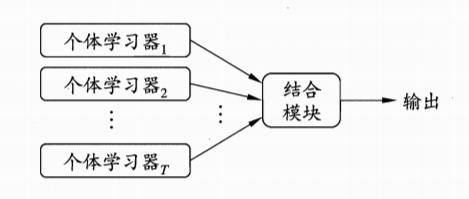
\includegraphics[width=0.5\linewidth]{fig/ensemble-learning.png}
\end{figure}

\subsection{Boosting}
提升(Boosting)可以将弱学习器提升为强学习器。

对目标函数$f(\vx)$进行多次逼近,通过不断拟合残差达到逼近的效果,可以按照下式不断迭代
\[\begin{aligned}
f_1(\vx) &=\widehat{f}(\vx)            & h_1(\vx) &=f(\vx)-f_1(\vx)\\
f_2(\vx) &=f_1(\vx)+\widehat{h_1}(\vx) & h_2(\vx) &=f(\vx)-f_2(\vx)\\
f_3(\vx) &=f_2(\vx)+\widehat{h_2}(\vx) & h_3(\vx) &=f(\vx)-f_3(\vx)\\
\vdots   &                             & \vdots \\
f_n(\vx) &=f_{n-1}(\vx)+\widehat{h_{n-1}}(\vx)
\end{aligned}\]

\subsection{Bagging与随机森林}
Bagging[Breiman, 1996]基于自助采样法,采样出$T$个含$m$个样本的采样集,然后基于每个采样集训练出一个基学习器,再将这些基学习器结合。

随机森林[Breiman, 2001]是Bagging的一个扩展变体。
传统决策树在选择划分属性时是在当前结点的属性集合(假定有$d$个属性)中选择一个最优属性;
而在随机森林中则是对基决策树的每个结点,先从该结点的属性集合中随机选择一个包含$k$个属性的子集,然后再从这个子集中选择一个最优属性进行划分。
这里的$k$即控制了随机程度,一般用$k=\log_2 d$[Breiman, 2001]。

\subsection{结合策略}
最简单的就是加权平均。

当训练数据很多时,更为强大的结合策略是使用学习法,即通过另一个学习器来进行结合。
Stacking[Wolpert, 1992]是学习法的典型代表。
这里把个体学习器称为次级学习器或元学习器(meta-learner)。

Stacking先从初始数据集中训练出初级学习器,然后生成一个新数据集用于训练次级学习器。
在新数据集中,初级学习器的输出被当作\emph{样例输入特征},而初始样本的标记仍被当作样例标记。

由于次级训练集是用初级学习器产生的,故直接用初级学习器的训练集产生次级学习器过拟合风险较大;因此常通过交叉验证或留一法,用训练初级学习器未使用的样本来产生次级学习器的训练样本。
以$k$折交叉验证为例,初始训练集$D$被随机划分为$k$个大小相似的集合$D_1,D_2,\ldots,D_k$。
令$D_j$和$\bar{D}_j=D\backslash D_j$分别表示第$j$折的测试集和训练集。
给定$T$个初级学习算法,初级学习器$h_t^{(j)}$通过在$\bar{D}_j$上使用第$t$个学习算法而得。
对于$D_j$的每个样本$\vx_i$,令$z_{it}=h_t^{(j)}(\vx_i)$,则由$\vx_i$所产生的次级训练样例的实例部分为$\vz_i=\bmat{z_{i1} & z_{i2} & \cdots & z_{iT}}$,标记部分为$y_i$。
故整个交叉验证过程结束后,从这$T$个初级学习器产生的次级训练集是$D'=\{(\vz_i,y_i\}_{i=1}^m$,然后$D'$将用于训练次级学习器。

贝叶斯模型平均(BMA)基于后验概率来为不同模型赋予权重,可视为加权平均的一种特殊实现。